\documentclass[thesis.tex]{subfiles}
\begin{document}

\appendix
\chapter{Histogram renormalization} \label{apx:histogramRenormalization}
%
This appendix chapter computes the equations needed to renormalize the bin aperture functions used in our histograms. We compute definite integrals from $a$ to $b$ of the box, triangle, and Gaussian kernel functions.
%
\section{Box kernel}
%
The box kernel with bin scale $\beta$ is defined as:
%
\begin{align*}
\mathit{Box} (x; \beta) = 
\begin{cases}
    \frac{1}{2 \beta},& \text{if } |x| \leq \beta \\
    0,              & \text{otherwise}
\end{cases}
\end{align*}
%
The kernel is only non-zero between $-\beta$ and $\beta$. Assuming $-\beta \leq a,b \leq \beta$,
%
\begin{align*}
\int_a^b \mathit{Box} (x; \beta) \,\mathrm dx &= \int_a^b \frac{1}{2 \beta} \,\mathrm dx \\
&= \frac{1}{2 \beta} (b - a)
\end{align*}
%
\section{Triangle kernel}
%
The triangle kernel with bin scale $\beta$ is defined as:
%
\begin{align*}
\mathit{Tri} (x; \beta) = 
\begin{cases}
    \frac{1}{2 \beta} \left( 1 - \frac{| x |}{2 \beta} \right) ,& \text{if } |x| \leq 2 \beta \\
    0,              & \text{otherwise}
\end{cases}
\end{align*}
%
The kernel is only non-zero between $-2\beta$ and $2\beta$. Assuming $-2 \beta \leq a \leq 0 \leq b \leq 2 \beta$,
%
\begin{align*}
\int_a^b \mathit{Tri} (x; \beta) \,\mathrm dx &= \frac{1}{2 \beta} \left( \int_a^0 \left( 1 + \frac{x}{2 \beta} \right) \,\mathrm dx + \int_0^b \left( 1 - \frac{x}{2 \beta} \right) \,\mathrm dx \right) \\
&= \frac{1}{2 \beta} \left( - a - \frac{a^2}{4 \beta} + b - \frac{b^2}{4 \beta} \right) \\
&= \frac{1}{2 \beta} (b - a) - \frac{1}{8 \beta^2} (a^2 + b^2)
\end{align*}
%
\section{Gaussian kernel}
\label{apx:gaussianKernel}
%
The Gaussian kernel with bin scale $\beta$ is defined as:
%
\begin{align*}
G(x;\beta) = \frac{1}{\sqrt{2\pi} \beta}
\exp\left( -\frac{x^2}{2 \beta^2} \right)
\end{align*}
%
The definite integral of $G(x;\beta)$ from $a$ to $b$ cannot be expressed by an elementary function. Instead we can use the non-elementary error function, defined as $\mathrm{erf}(b) = \frac{2}{\sqrt{\pi}} \int_0^b \exp(-x^2) \,\mathrm dx$, which can be computed by its Taylor series. First we show an intermediate result using the substitution $u = \sqrt{k} x$ with $\mathrm du = \sqrt{k} \mathrm dx$:
%
\begin{align*}
\int_0^b \exp(-k x^2) \,\mathrm dx
&= \frac{1}{\sqrt{k}} \int_0^{\sqrt{k}b} \exp(-u^2) \,\mathrm du \\
&= \frac{1}{\sqrt{k}} \frac{\sqrt{\pi}}{2} \mathrm{erf} \left( \sqrt{k} b \right)
\end{align*}
%
We use this to compute $\int_a^b G(x;\beta) \,\mathrm dx$:
%
\begin{align*}
\int_a^b G(x;\beta) \,\mathrm dx
&= \frac{1}{\sqrt{2\pi} \beta} \int_a^b \exp\left( -\frac{x^2}{2 \beta^2} \right) \,\mathrm dx \\
&= \frac{1}{\sqrt{2\pi} \beta} \left( \int_0^b \exp\left( -\frac{x^2}{2 \beta^2} \right) \,\mathrm dx - \int_0^a \exp\left( -\frac{x^2}{2 \beta^2} \right) \,\mathrm dx \right) \\
&= \frac{1}{\sqrt{2\pi} \beta} \frac{\sqrt{\pi}}{2} \sqrt{2} \beta \left(
\mathrm{erf} \left( \frac{1}{\sqrt{2} \beta} b \right) -
\mathrm{erf} \left( \frac{1}{\sqrt{2} \beta} a \right) \right) \\
&= \frac{1}{2} \left(
\mathrm{erf} \left( \frac{b}{\sqrt{2} \beta} \right) -
\mathrm{erf} \left( \frac{a}{\sqrt{2} \beta} \right)
\right)
\end{align*}
%
%The $n$-dimensional Gaussian filter with variances $\boldsymbol{\beta} = [\beta_1, ..., \beta_n]^T$ is defined as the product of $n$ 1-dimensional filters:
%%
%\begin{align*}
%G(\mathbf{x};\boldsymbol{\beta})
%&= \prod_i G(x_i;\beta_i) \\
%&= \frac{1}{(2\pi)^\frac{n}{2} \prod_i \mathbf{\beta}_i}
%\exp\left( -\sum_i \frac{x_i^2}{2 \beta_i^2} \right)
%\end{align*}
%%
%With this definition we disallow arbitrary covariances as it does not make sense for a binning function. Note that the factors of $G(\mathbf{x};\boldsymbol{\beta})$ contain distinct variables. Thus its definite integral from $a_i$ to $b_i$ in each dimension is simply the product of the definite integrals for each dimension:
%%
%\begin{align*}
%\int_{a_i}^{b_i} \dots \int_{a_n}^{b_n} G(\mathbf{x},\boldsymbol{\beta}) \,\mathrm d{x_n} \dots d{x_i}
%&= \prod_i \int_{a_i}^{b_i} G(\mathbf{x},\boldsymbol{\beta}) \,\mathrm d{x_i} \\
%&= \prod_i \frac{1}{2} \left(
%\mathrm{erf} \left( \frac{b_i}{\sqrt{2} \beta_i} \right) -
%\mathrm{erf} \left( \frac{a_i}{\sqrt{2} \beta_i} \right)
%\right)
%\end{align*}
%
\chapter{Image transformations} \label{apx:image_transformations}

Recall the definitions of gradient orientation $\Theta$, gradient magnitude $M$, shape index $S$, and curvedness $C$ defined in \Cref{sec:diffStructure}.
This appendix chapter computes the effect of certain image transformations on the mentioned functions.

\section{Rotation} \label{apx:rotation}

Let $\widetilde{L}$ be the blurred image $L$ rotated around some point $\mathbf{x}$ by angle $\theta$. That is, we rotate the original coordinate system axes $\mathbf{e}_x, \mathbf{e}_y$ by multiplying by a rotation matrix $\mathbf{R}$:
%
\begin{align*}
\mathbf{R} &= \begin{bmatrix}
\cos \theta & -\sin \theta \\
\sin \theta & \cos \theta
\end{bmatrix} \\
\mathbf{Re}_x &= \begin{bmatrix}
\cos \theta \\ \sin \theta
\end{bmatrix} \\
\mathbf{Re}_y &= \begin{bmatrix}
-\sin \theta \\ \cos \theta
\end{bmatrix}
\end{align*}
%
Now the first and second order derivatives can be computed by directional derivatives along the coordinate system axes:
%
\begin{align*}
L_i &= \nabla_{\mathbf{e}_i} L \\
\widetilde{L}_i &= \nabla_{\mathbf{Re}_i} L = (\mathbf{Re}_i)^T \nabla L \\
\widetilde{L}_x &= \cos \theta L_x + \sin \theta L_y \\
\widetilde{L}_y &= -\sin \theta L_x + \cos \theta L_y \\
L_{ij} &= \nabla_{\mathbf{e}_i} (\nabla_{\mathbf{e}_j} L) \\
\widetilde{L}_{ij} &= \nabla_{\mathbf{Re}_i} (\nabla_{\mathbf{Re}_j} L)
= \nabla_{\mathbf{Re}_i} \left( (\mathbf{Re}_j)^T \nabla L \right)
= (\mathbf{Re}_j)^T \nabla^2 L (\mathbf{Re}_i) \\
\widetilde{L}_{xx} &= \cos^2 \theta L_{xx} + \sin^2 \theta L_{yy} + 2 \cos \theta \sin \theta L_{xy} \\
&= \cos^2 \theta L_{xx} + \sin^2 \theta L_{yy} + \sin 2\theta L_{xy} \\
\widetilde{L}_{yy} &= \sin^2 \theta L_{xx} + \cos^2 \theta L_{yy} - 2 \cos \theta \sin \theta L_{xy} \\
&= \sin^2 \theta L_{xx} + \cos^2 \theta L_{yy} - \sin 2\theta L_{xy} \\
\widetilde{L}_{xy} &= -\cos \theta \sin \theta L_{xx} + (\cos^2 \theta - \sin^2 \theta) L_{xy} + \cos \theta \sin \theta L_{yy} \\
&= -\frac12 \sin 2\theta (L_{xx} - L_{yy}) + \cos 2\theta L_{xy}
\end{align*}
%
\subsection{Gradient orientation} \label{apx:rotation_go}
%
First we show an intermediate result using a common tangent identity:
%
\begin{align*}
\tan \left( \Atan{\frac{L_y}{L_x}} - \theta \right)
&= \frac{\tan \left( \Atan{\frac{L_y}{L_x}} \right) - \tan \theta}{1 + \tan \left( \Atan{\frac{L_y}{L_x}} \right) \tan \theta} \\
&= \frac{\frac{L_y}{L_x} - \frac{\sin \theta}{\cos \theta}}{1 + \frac{L_y}{L_x} \frac{\sin \theta}{\cos \theta}} \\
&= \frac{\left(\frac{-\sin \theta L_x + \cos \theta L_y}{L_x \cos \theta}\right)}{\left(\frac{\cos \theta L_x + \sin \theta L_y}{L_x \cos \theta}\right)} \\
&= \frac{-\sin \theta L_x + \cos \theta L_y}{\cos \theta L_x + \sin \theta L_y}
\end{align*}
%
We use this to compute the transformed gradient orientation $\widetilde{\Theta}$:
%
\begin{align*}
\widetilde{\Theta} &= \Atan{\frac{\widetilde{L}_y}{\widetilde{L}_x}} \\
&= \Atan{\frac{-\sin \theta L_x + \cos \theta L_y}{\cos \theta L_x + \sin \theta L_y}} \\
&= \Atan{\frac{L_y}{L_x}} - \theta = \Theta - \theta
\end{align*}
%
\subsection{Gradient magnitude} \label{apx:rotation_m}
We here compute the transformed gradient magnitude $\widetilde{M}$:
%
\begin{align*}
\widetilde{M} &= \sqrt{\widetilde{L}_x^2 + \widetilde{L}_y^2} \\
&= \sqrt{(\cos \theta L_x + \sin \theta L_y)^2 + (-\sin \theta L_x + \cos \theta L_y)^2} \\
&= \sqrt{L_x^2 + L_y^2} = M
\end{align*}
%
\subsection{Shape index} \label{apx:rotation_si}
%
Define $S_n = -L_{xx} - L_{yy}$ and $S_d = 4 L_{xy}^2 + (L_{xx} - L_{yy})^2$ such that the shape index is defined as $S = \frac{2}{\pi} \Atan{S_n/\sqrt{S_d}}$.

We first define the transformed nominator $\widetilde{S}_n$ and denominator $\widetilde{S}_d$ to show that $\widetilde{S}_n = S_n$ and $\widetilde{S}_d = S_d$:
%
\begin{align*}
\widetilde{S}_n &= - \widetilde{L}_{xx} - \widetilde{L}_{yy} \\
&= -(\cos^2 \theta + \sin^2 \theta)  L_{xx} - (\cos^2 \theta + \sin^2 \theta) L_{yy} \\
&= -L_{xx} - L_{yy} = S_n \\
4\widetilde{L}_{xy}^2 &= 4(-\frac12 \sin 2\theta (L_{xx} - L_{yy}) + \cos 2\theta L_{xy})^2 \\
&= (- \sin 2\theta (L_{xx} - L_{yy}) + 2 \cos 2\theta L_{xy})^2 \\
(\widetilde{L}_{xx} - \widetilde{L}_{yy})^2 &= ((\cos^2 \theta - \sin^2 \theta) (L_{xx} - L_{yy}) + 2 \sin 2\theta L_{xy})^2 \\
&= (\cos 2\theta (L_{xx} - L_{yy}) + 2 \sin 2\theta L_{xy})^2 \\
\widetilde{S}_d &= 4\widetilde{L}_{xy}^2 + (\widetilde{L}_{xx} - \widetilde{L}_{yy})^2 \\
&= (\sin^2 2\theta - \cos^2 2\theta) (L_{xx} - L_{yy})^2 + 4 (\cos^2 2\theta + \sin^2 2\theta) L_{xy}^2 \\
&= 4 L_{xy}^2 + (L_{xx} - L_{yy})^2 = S_d
\end{align*}
%
And thus $\widetilde{S} = S$.
%
\subsection{Curvedness} \label{apx:rotation_c}
Let $\widetilde{L}_{xx}$ and $\widetilde{L}_{yy}$ be the transformed $L_{xx}$ and $L_{yy}$, and $\widetilde{C}$ be the transformed curvedness.
%
\begin{align*}
\widetilde{L}_{xx}^2 + \widetilde{L}_{yy}^2
&= (\cos^4 \theta + \sin^4 \theta) (L_{xx}^2 + L_{yy}^2) + 2 \sin^2 2\theta L_{xy}^2 \\ &\qquad + \sin^2 2\theta L_{xx} L_{yy} + \sin 4\theta (L_{xx} - L_{yy}) L_{xy} \\
2 \widetilde{L}_{xy}^2 &= \frac12 \sin^2 2\theta (L_{xx} - L_{yy})^2 + 2 \cos^2 2\theta L_{xy}^2 - \sin 4\theta (L_{xx} - L_{yy}) L_{xy} \\
\widetilde{L}_{xx}^2 + \widetilde{L}_{yy}^2 + 2 \widetilde{L}_{xy}^2
&= (\cos^4 \theta + \sin^4 \theta) (L_{xx}^2 + L_{yy}^2) + \sin^2 2\theta L_{xx} L_{yy} \\ &\qquad + \frac12 \sin^2 2\theta (L_{xx} - L_{yy})^2 + 2 L_{xy} \\
&= (\cos^4 \theta + \sin^4 \theta) (L_{xx}^2 + L_{yy}^2) + \frac12 \sin^2 2\theta (L_{xx}^2 + L_{yy}^2) + 2 L_{xy} \\
&= (\cos^2 \theta + \sin^2 \theta)^2 (L_{xx}^2 + L_{yy}^2) + 2 L_{xy} \\
&= L_{xx}^2 + L_{yy}^2 + 2 L_{xy}
\end{align*}
%
and thus
%
\begin{align*}
\widetilde{C} &= \frac12 \sqrt{\widetilde{L}_{xx}^2 + 2 \widetilde{L}_{xy}^2 + \widetilde{L}_{yy}^2} = C
\end{align*}
%
\section{Illumination} \label{apx:illumination}
%
Under the assumption of an affine illumination model $\widetilde{I} = aI + b$ where $I$ is the underlying image, the four transformed measures $\widetilde{\Theta}$, $\widetilde{M}$, $\widetilde{S}$ and $\widetilde{C}$ are computed:
%
\begin{align*}
  \widetilde{L}_{x^m y^n} &= a L_{x^m y^n}, \quad m+n > 0 \\
  \widetilde{\Theta} &= \Atan{\frac{a L_y}{a L_x}} = \Atan{\frac{L_y}{L_x}} = \Theta \\
  \widetilde{M} &= \sqrt{(a L_x)^2 + (a L_y)^2} = a \sqrt{L_x^2 + L_y^2} = a M \\
  \widetilde{S} &= \frac{2}{\pi} \Atan{\frac{-a L_{xx} - a L_{yy}}{\sqrt{4(aL_{xy})^2 + (aL_{xx} - aL_{yy})^2}}} \\
  &= \frac{2}{\pi} \Atan{\frac{a (-L_{xx} - L_{yy})}{\sqrt{a^2 \left(4L_{xy}^2 + \left(L_{xx} - L_{yy} \right)^2 \right)}}} \\
  &= \frac{2}{\pi} \Atan{\frac{-L_{xx} - L_{yy}}{\sqrt{4L_{xy}^2 + \left(L_{xx} - L_{yy} \right)^2}}} = S \\
  \widetilde{C} &= \frac12 \sqrt{(a L_{xx})^2 + 2 (a L_{xy})^2 + (a L_{yy})^2} \\
  &= \frac12 a \sqrt{L_{xx}^2 + 2 L_{xy}^2 + L_{yy}^2} = a C
\end{align*}
%
%When normalizing $k$-jet with $L_2$-norm:
%
%\begin{align*}
%  \mathcal{J}_k &= \left( \mset{L_{x^n y^m} | 0 < n+m \leq k} \right)^T \\
%  \widetilde{\mathcal{J}}_k &=\left( \mset{a L_{x^n y^m} | 0 < n+m \leq k} \right)^T \\
%  \left \| \widetilde{\mathcal{J}}_k \right \|_2 &= \sqrt{\sum_{0 < n+m \leq k} (a L_{x^n y^m})^2} \\
%      &= \sqrt{a^2\sum_{0 < n+m \leq k} (L_{x^n y^m})^2} \\
%      &= a\sqrt{\sum_{0 < n+m \leq k} (L_{x^n y^m})^2} \\
%      &= a \left \| \mathcal{J}_k \right \|_2 \\
%  \frac{\widetilde{\mathcal{J}}_k}{\left \| \widetilde{\mathcal{J}}_k \right \|_2} &=
%      \frac{\mathcal{J}_k}{\left \| \mathcal{J}_k \right \|_2}
%\end{align*}

\chapter{Grid layouts}
\label{apx:gridLayouts}
%
This appendix chapter describes the construction of our log-polar grid layouts shown in \Cref{fig:gridType}. They consist of a central cell as well as a constant number of Gaussian cells in each of a number of rings, where the cells' standard deviations (referred to as radii) are tangent to each other and thus non-overlapping. We define $r_i$ to be the radius of a cell in ring $i$, and $d_i$ to be its distance from the origin.
%
\section{Log-polar grids}
%
We consider two tangent cells from neighbouring rings in the log-polar grid, which will be sufficient to construct the whole grid:
%
\begin{figure}[H]
	\centering
	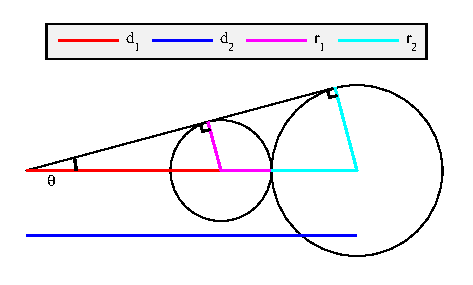
\includegraphics[width=\textwidth]{img/gridLayoutDerivationNormal.pdf}
   	\caption{Log-polar grid layout.}
  	\label{fig:gridLayoutDerivationNormal}
\end{figure}
\noindent
%
First we compute the relation between $r_i$ and $d_i$. As we have a right-angled triangle, we can use the sine definition:
%
\begin{align}
\sin \theta = \frac{r_i}{d_i}
\label{eq:radiusDistanceRelation}
\end{align}
%
Note that this linear dependency holds for any ring $i$. Thus, with the grid definition, the only thing left is to compute the relation between two neighbouring rings, which we can write as the constant $k$ such that $r_{i+1} = k r_i$ and $d_{i+1} = k d_i$. We compute $k$:
%
\begin{align*}
d_2 = k d_1 &= d_1 + r_1 + r_2 = d_1 + d_1 \sin \theta + k d_1 \sin \theta \quad\Rightarrow \\
k - k \sin \theta &= 1 + \sin \theta \quad\Rightarrow \\
k &= \frac{1 + \sin \theta}{1 - \sin \theta}
\end{align*}
%
Now the whole log-polar grid can be constructed. A circle is added to the middle as the central cell, and the whole grid is rescaled according to the desired radius.
%
\section{Concentric log-polar grids}
%
We again consider two tangent cells from neighbouring rings, this time offset by the angle $\theta$, causing a different layout:
%
\begin{figure}[H]
	\centering
	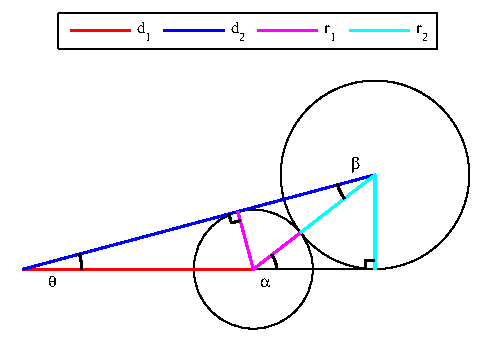
\includegraphics[width=\textwidth]{img/gridLayoutDerivationConcentric.pdf}
    \caption{Concentric log-polar grid layout.}
    \label{fig:gridLayoutDerivationConcentric}
\end{figure}
\noindent
%
Note that \Cref{eq:radiusDistanceRelation} still holds for this grid. The constant $k$ however is more complicated to compute. First note that the supplementary angle to $\alpha$ together with $\theta$ and $\beta$ must add up to $180^\circ$, so $\alpha = \theta + \beta$. We use the sine definition with two of the right-angled triangles:
%
\begin{align}
\sin (\theta + \beta) &= \frac{r_2}{r_1 + r_2} \nonumber \\
\sin \beta &= \frac{r_1}{r_1 + r_2} \label{eq:kFromBeta}
\end{align}
%
Added together this gives
%
\begin{align*}
\sin (\theta + \beta) + \sin \beta = \frac{r_1 + r_2}{r_1 + r_2} = 1
\end{align*}
%
which is sufficient to calculate $\beta$ by symbolic computation, but the result is quite ugly. Then $k$ can be computed from \Cref{eq:kFromBeta}:
%
\begin{align*}
\sin \beta &= \frac{1}{1 + k} \quad\Rightarrow \\
k &= \frac{1}{\sin \beta} - 1
\end{align*}
%
Now the whole concentric log-polar grid can be constructed alike the ordinary log-polar grid.
%
\chapter{Gaussian derivatives}
%
The $n$'th order derivative of the 1D Gaussian kernel $G$ has the following relation to the Hermite polynomial:
%
\begin{align*}
	G_{x^n}(x;\sigma) &= \left(\frac{1}{\sqrt{2}\sigma}\right)^n \cdot
						 \frac{1}{\sqrt{2\pi}\sigma} \cdot
						 \exp \left( \frac{x^2}{2\sigma^2} \right) \cdot
						 \text{hermite} \left(n,\frac{x^2}{\sqrt{2}\sigma} \right)
\end{align*}
%
Thus an arbitrary 2D Gaussian derivative with equal variance in both dimensions can be written as:
%
\begin{align*}
	G_{x^m y^n}(x,y;\sigma) &=
						G_{y^n}(y;\sigma)^\text{T} \ast G_{x^m}(x;\sigma)
\end{align*}

\chapter{Confidence intervals for image correspondence}
\label{apx:confidenceIntervals}
In this appendix chapter we show the 95\% confidence interval graphs for the difference between mean performance on the DTU dataset paths of two descriptors. \Cref{fig:dtuResultsStatsGo_GoSi,fig:dtuResultsStatsSi_GoSi,fig:dtuResultsStatsGo_Si,fig:dtuResultsStatsGo_Sift,fig:dtuResultsStatsSi_Sift} shown the graphs for the combinations of the GO, SI, GO+SI and SIFT descriptors. The combination GO+SI and SIFT is left out since it is shown directly in the report in \Cref{fig:dtuResultsStats}.

\begin{figure}[tb]
	\centerline{
	\begin{subfigure}[t]{0.6242\textwidth}
		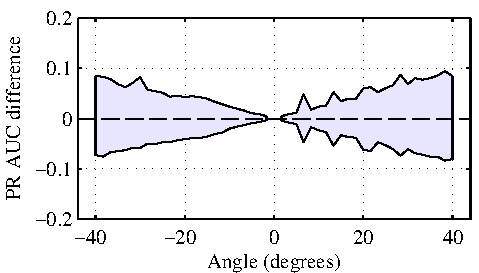
\includegraphics[width=\textwidth]{img/dtuResultsStatsGoSi_Go_1.pdf}
		\caption{Arc 1}
	\end{subfigure}
	\begin{subfigure}[t]{0.5618\textwidth}
		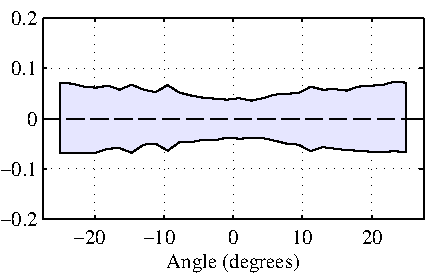
\includegraphics[width=\textwidth]{img/dtuResultsStatsGoSi_Go_2.pdf}
		\caption{Arc 2}
	\end{subfigure}
	}
	\centerline{
	\begin{subfigure}[t]{0.6242\textwidth}
		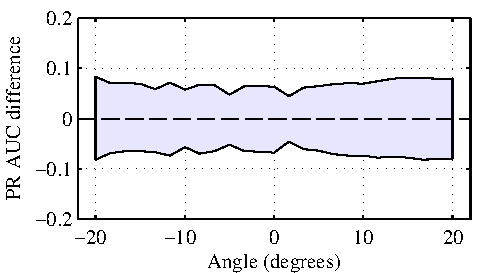
\includegraphics[width=\textwidth]{img/dtuResultsStatsGoSi_Go_3.pdf}
		\caption{Arc 3}
	\end{subfigure}
	\begin{subfigure}[t]{0.5618\textwidth}
		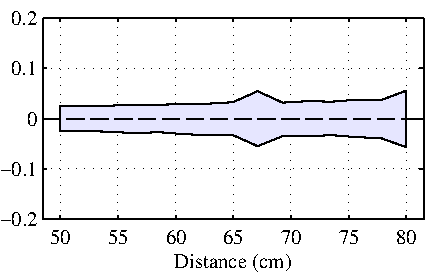
\includegraphics[width=\textwidth]{img/dtuResultsStatsGoSi_Go_4.pdf}
		\caption{Linear path}
	\end{subfigure}
	}
	\centerline{
	\begin{subfigure}[t]{0.6242\textwidth}
		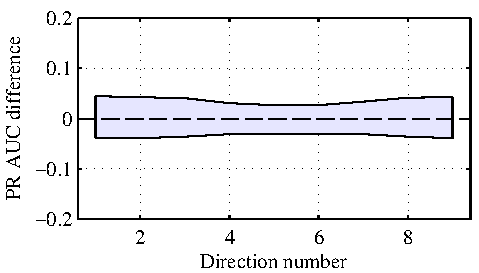
\includegraphics[width=\textwidth]{img/dtuResultsStatsGoSi_Go_5.pdf}
		\caption{Light path, $x$-axis}
	\end{subfigure}
	\begin{subfigure}[t]{0.5618\textwidth}
		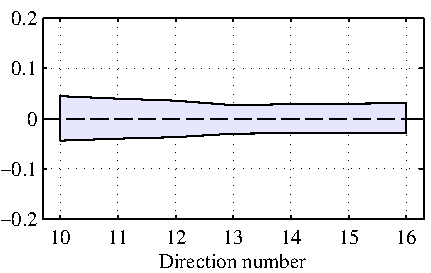
\includegraphics[width=\textwidth]{img/dtuResultsStatsGoSi_Go_6.pdf}
		\caption{Light path, $z$-axis}
	\end{subfigure}
	}
	\caption{95\% confidence intervals on the PR AUC difference between our GO+SI and GO descriptors. A positive difference denotes that GO+SI outperforms GO and vise versa. If the confidence interval for a position contains zero, there is no significant difference in performance.}
	\label{fig:dtuResultsStatsGo_GoSi}
\end{figure}

\begin{figure}[tb]
	\centerline{
	\begin{subfigure}[t]{0.6242\textwidth}
		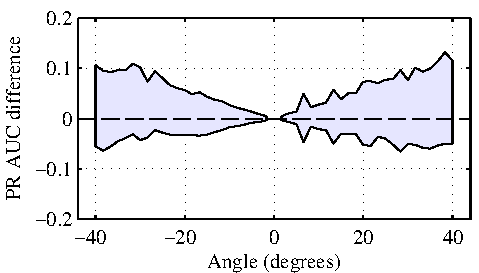
\includegraphics[width=\textwidth]{img/dtuResultsStatsGoSi_Si_1.pdf}
		\caption{Arc 1}
	\end{subfigure}
	\begin{subfigure}[t]{0.5618\textwidth}
		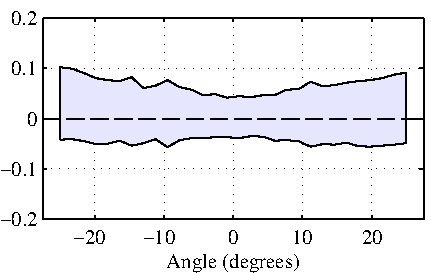
\includegraphics[width=\textwidth]{img/dtuResultsStatsGoSi_Si_2.pdf}
		\caption{Arc 2}
	\end{subfigure}
	}
	\centerline{
	\begin{subfigure}[t]{0.6242\textwidth}
		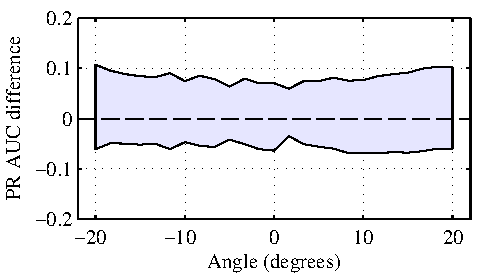
\includegraphics[width=\textwidth]{img/dtuResultsStatsGoSi_Si_3.pdf}
		\caption{Arc 3}
	\end{subfigure}
	\begin{subfigure}[t]{0.5618\textwidth}
		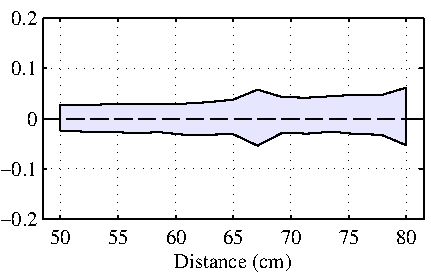
\includegraphics[width=\textwidth]{img/dtuResultsStatsGoSi_Si_4.pdf}
		\caption{Linear path}
	\end{subfigure}
	}
	\centerline{
	\begin{subfigure}[t]{0.6242\textwidth}
		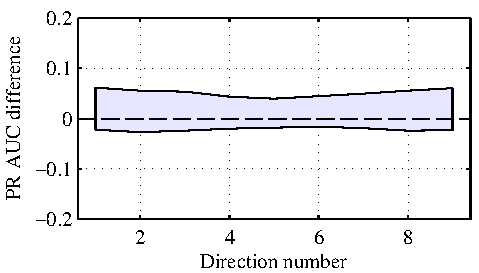
\includegraphics[width=\textwidth]{img/dtuResultsStatsGoSi_Si_5.pdf}
		\caption{Light path, $x$-axis}
	\end{subfigure}
	\begin{subfigure}[t]{0.5618\textwidth}
		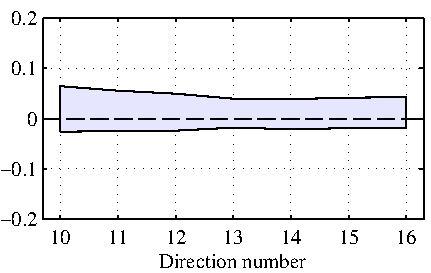
\includegraphics[width=\textwidth]{img/dtuResultsStatsGoSi_Si_6.pdf}
		\caption{Light path, $z$-axis}
	\end{subfigure}
	}
	\caption{95\% confidence intervals on the PR AUC difference between our GO+SI and SI descriptors. A positive difference denotes that GO+SI outperforms SI and vise versa. If the confidence interval for a position contains zero, there is no significant difference in performance.}
	\label{fig:dtuResultsStatsSi_GoSi}
\end{figure}


\begin{figure}[tb]
	\centerline{
	\begin{subfigure}[t]{0.6242\textwidth}
		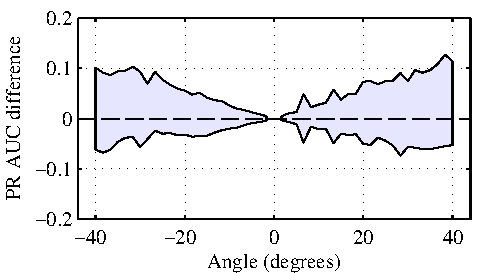
\includegraphics[width=\textwidth]{img/dtuResultsStatsGo_Si_1.pdf}
		\caption{Arc 1}
	\end{subfigure}
	\begin{subfigure}[t]{0.5618\textwidth}
		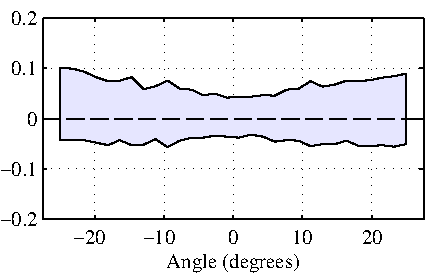
\includegraphics[width=\textwidth]{img/dtuResultsStatsGo_Si_2.pdf}
		\caption{Arc 2}
	\end{subfigure}
	}
	\centerline{
	\begin{subfigure}[t]{0.6242\textwidth}
		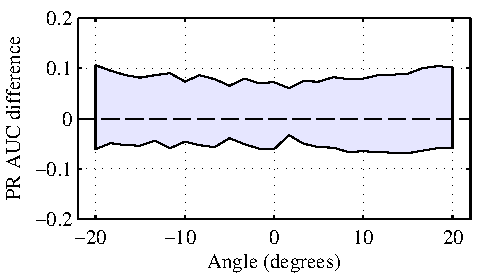
\includegraphics[width=\textwidth]{img/dtuResultsStatsGo_Si_3.pdf}
		\caption{Arc 3}
	\end{subfigure}
	\begin{subfigure}[t]{0.5618\textwidth}
		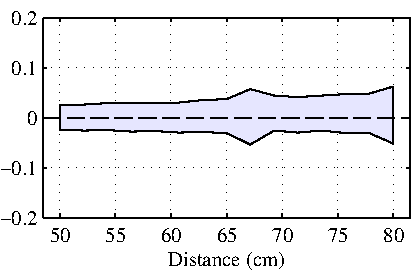
\includegraphics[width=\textwidth]{img/dtuResultsStatsGo_Si_4.pdf}
		\caption{Linear path}
	\end{subfigure}
	}
	\centerline{
	\begin{subfigure}[t]{0.6242\textwidth}
		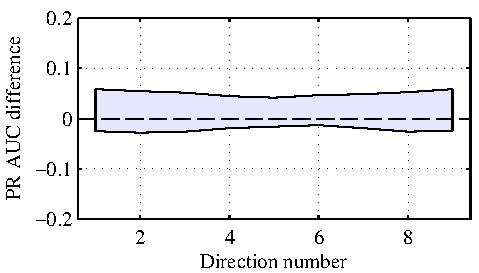
\includegraphics[width=\textwidth]{img/dtuResultsStatsGo_Si_5.pdf}
		\caption{Light path, $x$-axis}
	\end{subfigure}
	\begin{subfigure}[t]{0.5618\textwidth}
		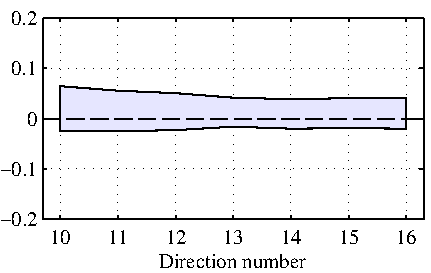
\includegraphics[width=\textwidth]{img/dtuResultsStatsGo_Si_6.pdf}
		\caption{Light path, $z$-axis}
	\end{subfigure}
	}
	\caption{95\% confidence intervals on the PR AUC difference between our GO and SI descriptors. A positive difference denotes that GO outperforms SI and vice versa. If the confidence interval for a position contains zero, there is no significant difference in performance.}
	\label{fig:dtuResultsStatsGo_Si}
\end{figure}


\begin{figure}[tb]
	\centerline{
	\begin{subfigure}[t]{0.6242\textwidth}
		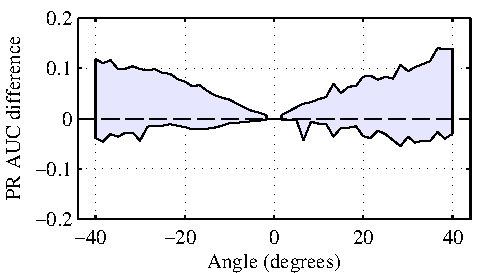
\includegraphics[width=\textwidth]{img/dtuResultsStatsGo_Sift_1.pdf}
		\caption{Arc 1}
	\end{subfigure}
	\begin{subfigure}[t]{0.5618\textwidth}
		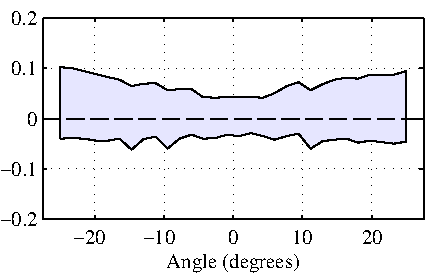
\includegraphics[width=\textwidth]{img/dtuResultsStatsGo_Sift_2.pdf}
		\caption{Arc 2}
	\end{subfigure}
	}
	\centerline{
	\begin{subfigure}[t]{0.6242\textwidth}
		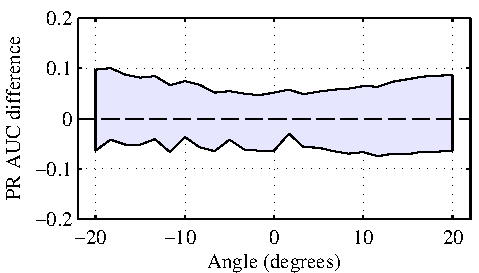
\includegraphics[width=\textwidth]{img/dtuResultsStatsGo_Sift_3.pdf}
		\caption{Arc 3}
	\end{subfigure}
	\begin{subfigure}[t]{0.5618\textwidth}
		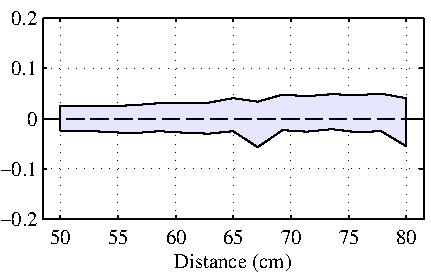
\includegraphics[width=\textwidth]{img/dtuResultsStatsGo_Sift_4.pdf}
		\caption{Linear path}
	\end{subfigure}
	}
	\centerline{
	\begin{subfigure}[t]{0.6242\textwidth}
		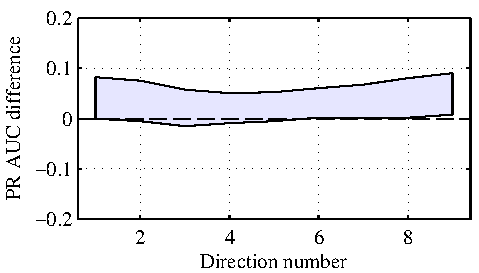
\includegraphics[width=\textwidth]{img/dtuResultsStatsGo_Sift_5.pdf}
		\caption{Light path, $x$-axis}
	\end{subfigure}
	\begin{subfigure}[t]{0.5618\textwidth}
		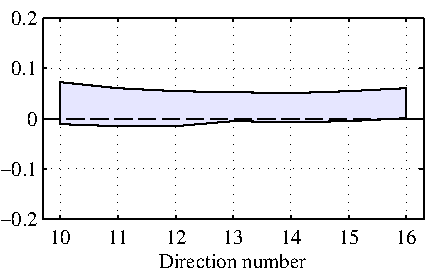
\includegraphics[width=\textwidth]{img/dtuResultsStatsGo_Sift_6.pdf}
		\caption{Light path, $z$-axis}
	\end{subfigure}
	}
	\caption{95\% confidence intervals on the PR AUC difference between our GO descriptor and SIFT. A positive difference denotes that GO outperforms SIFT and vise versa. If the confidence interval for a position contains zero, there is no significant difference in performance.}
	\label{fig:dtuResultsStatsGo_Sift}
\end{figure}

\begin{figure}[tb]
	\centerline{
	\begin{subfigure}[t]{0.6242\textwidth}
		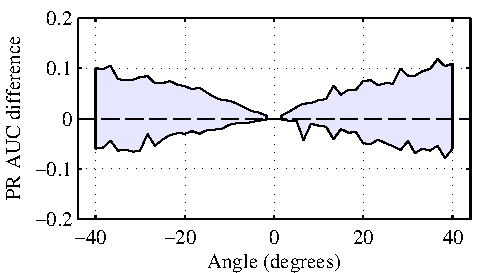
\includegraphics[width=\textwidth]{img/dtuResultsStatsSi_Sift_1.pdf}
		\caption{Arc 1}
	\end{subfigure}
	\begin{subfigure}[t]{0.5618\textwidth}
		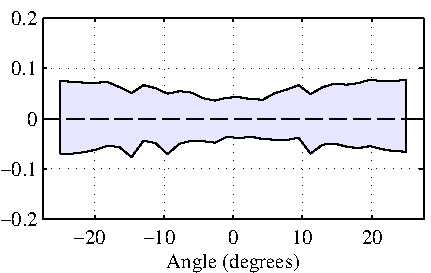
\includegraphics[width=\textwidth]{img/dtuResultsStatsSi_Sift_2.pdf}
		\caption{Arc 2}
	\end{subfigure}
	}
	\centerline{
	\begin{subfigure}[t]{0.6242\textwidth}
		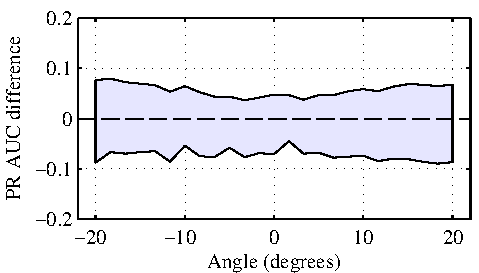
\includegraphics[width=\textwidth]{img/dtuResultsStatsSi_Sift_3.pdf}
		\caption{Arc 3}
	\end{subfigure}
	\begin{subfigure}[t]{0.5618\textwidth}
		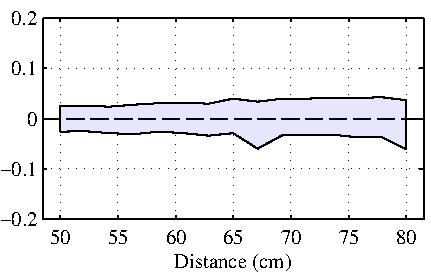
\includegraphics[width=\textwidth]{img/dtuResultsStatsSi_Sift_4.pdf}
		\caption{Linear path}
	\end{subfigure}
	}
	\centerline{
	\begin{subfigure}[t]{0.6242\textwidth}
		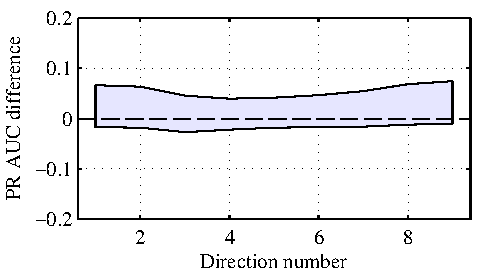
\includegraphics[width=\textwidth]{img/dtuResultsStatsSi_Sift_5.pdf}
		\caption{Light path, $x$-axis}
	\end{subfigure}
	\begin{subfigure}[t]{0.5618\textwidth}
		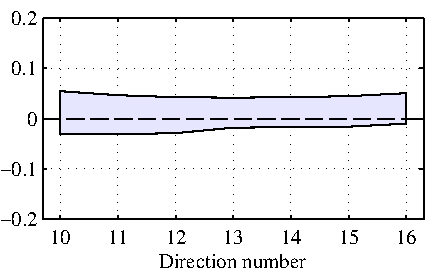
\includegraphics[width=\textwidth]{img/dtuResultsStatsSi_Sift_6.pdf}
		\caption{Light path, $z$-axis}
	\end{subfigure}
	}
	\caption{95\% confidence intervals on the PR AUC difference between our SI descriptor and SIFT. A positive difference denotes that SI outperforms SIFT and vise versa. If the confidence interval for a position contains zero, there is no significant difference in performance.}
	\label{fig:dtuResultsStatsSi_Sift}
\end{figure}

\subbibliography

\end{document}
